\documentclass{article}
\usepackage{tikz}

\begin{document}

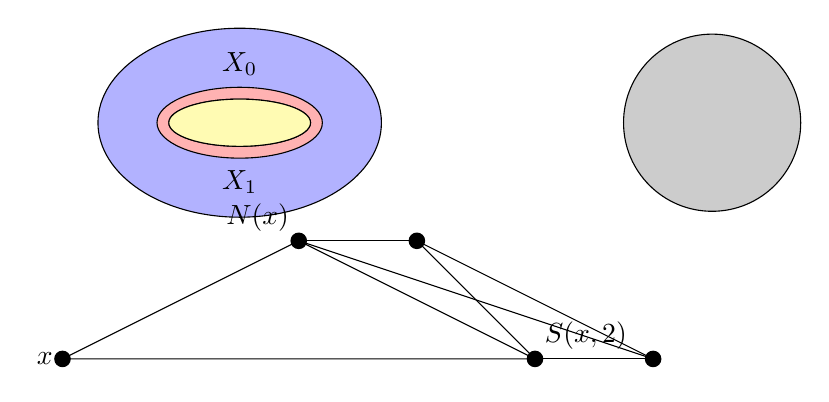
\begin{tikzpicture}[scale=1.5]
    % Define points
    \coordinate (x) at (-2, 0);
    \coordinate (y) at (0, 1);
    \coordinate (z) at (2, 0);
    \coordinate (y') at (1, 1);
    \coordinate (z') at (3, 0);

    % Draw circles
    \draw[fill=gray!40] (-0.5, 2) circle (0.75);
    \draw[fill=gray!40] (3.5, 2) circle (0.75);
    \draw[fill=blue!30] (-0.5, 2) ellipse (1.2 and 0.8); % X_0
    \draw[fill=red!30] (-0.5, 2) ellipse (0.7 and 0.3); % X_0 (center)
    \draw[fill=red!30] (-0.5, 2) ellipse (0.6 and 0.2); % X_1 (center)
    \draw[fill=yellow!30] (-0.5, 2) ellipse (0.6 and 0.2); % X_1 (center)

    % Draw lines
    \draw (x) -- (y) -- (z) -- (x);
    \draw (y) -- (y');
    \draw (z) -- (z');
    \draw (y') -- (y);
    \draw (z') -- (z);
    \draw (y') -- (z');
    \draw (y') -- (z);
    \draw (z') -- (y);

    % Label points
    \fill (x) circle (2pt) node[left] {$x$};
    \fill (y) circle (2pt) node[above left] {$N(x)$};
    \fill (z) circle (2pt) node[above right] {$S(x, 2)$};
    \fill (y') circle (2pt) node[right] {};
    \fill (z') circle (2pt) node[right] {};

    % Set labels
    \node at (-0.5, 2.5) {$X_0$};
    \node at (-0.5, 1.5) {$X_1$};
\end{tikzpicture}

\end{document}